\chapter{Разработка КИМ пространственной модели и исследование динамики управления ОЭП при действии возмущений} \label{ch:ch5}

\section{КИМ трехфазного моментного привода} \label{ch:ch5/sect1}

Используя уравнения полученые в разделе \ref{ch:ch3/sect9} составим компьютерную модель привода.

В соответствии с системой уравнений (\ref{eq:p3:9.1}) составим структурную схему привода:
\begin{figure}[ht]
	\centering
	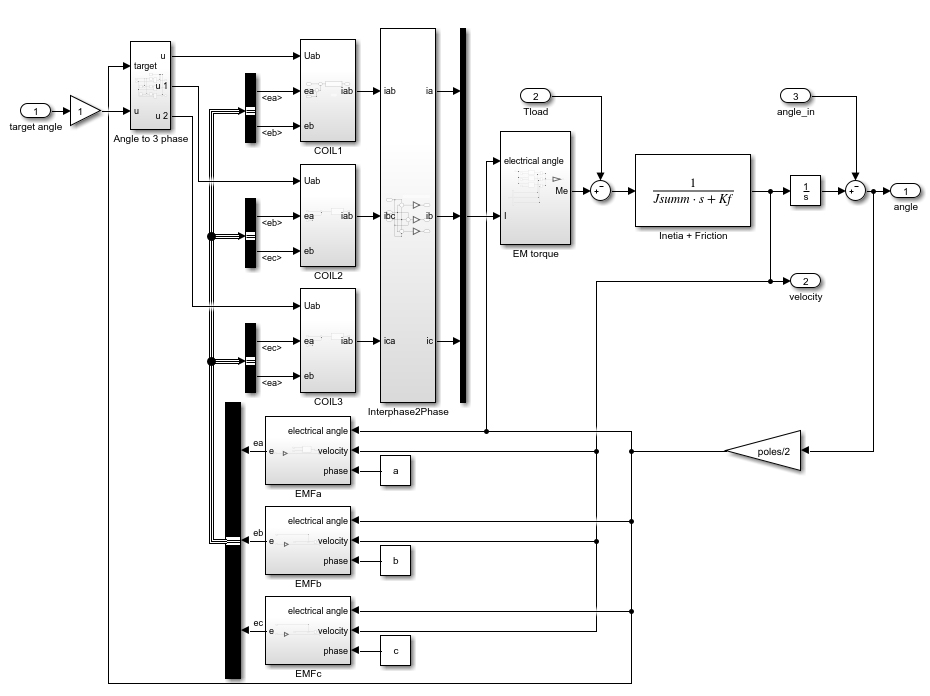
\includegraphics[width=1.0\linewidth]{motor} 
	\caption{Схема модели трехфазного ДБМ}
	\label{fig:motor}
\end{figure}

Часть уравнения учитывающая зависимость напряжения фазы от тока описывается блоком COILx, где номер фазы. Структура блока показан на рисунке \ref{fig:motor_coil}.

\begin{figure}[ht]
	\centering
	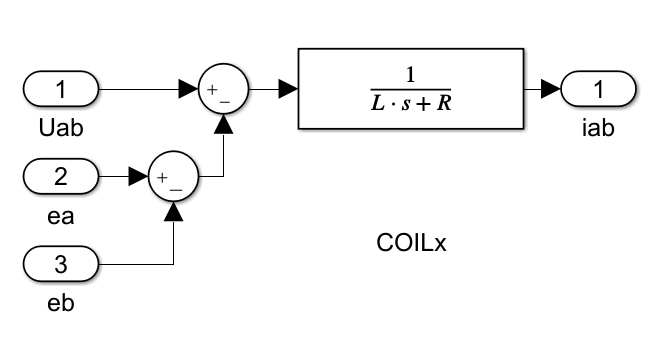
\includegraphics[width=0.6\linewidth]{coil} 
	\caption{Схема блока COILx}
	\label{fig:motor_coil}
\end{figure}

Для преобразования межфазных токов в фазовые введен блок "Interphase2Phase", его структура показана на рисунке \ref{fig:CC}.

\begin{figure}[ht]
	\centering
	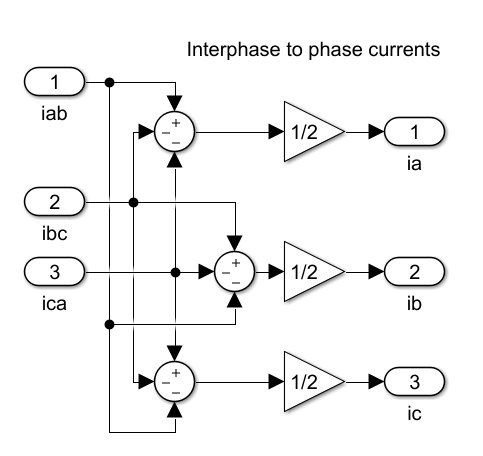
\includegraphics[width=0.4\linewidth]{CC} 
	\caption{Схема пересчета токов}
	\label{fig:CC}
\end{figure}

Уравнение (\ref{eq:p3:9.4}) реализовано в блоке моделирующем электромагнитный крутящий момент силы привода (рисунок \ref{fig:EMT}).

\begin{figure}[ht]
	\centering
	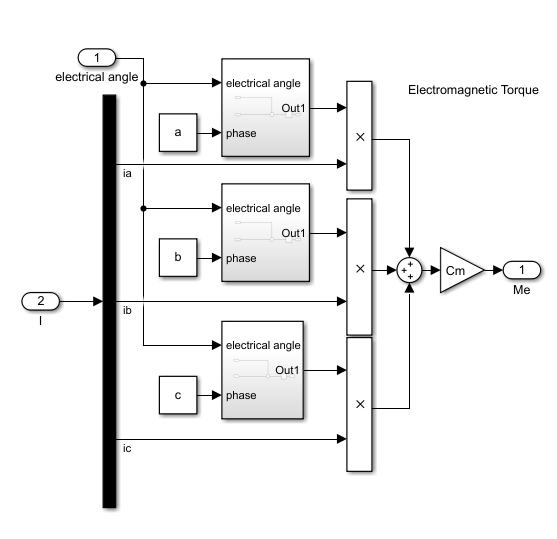
\includegraphics[width=0.6\linewidth]{EMT} 
	\caption{Блок моделирования электромагнитного крутящего момента силы привода}
	\label{fig:EMT}
\end{figure}

Пользуясь уравнением (\ref{eq:p4:s3.1}) или его нелинеаризованной формой (\ref{eq:p3:49}) можно вычислить угловую скорость для определения обратнонаведенного ЭДС, участвующую в уравнении (\ref{eq:p3:9.1}). Уравнение связывающее угловую скорость привода и обратнонаведенную ЭДС, описанное формулой (\ref {eq:p3:9.2}), моделируется блоком EMFx (рисунок \ref{fig:EMF}).

\begin{figure}[ht]
	\centering
	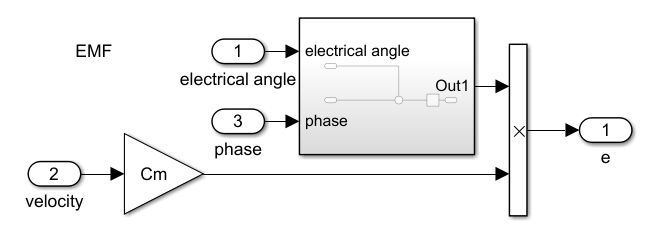
\includegraphics[width=0.5\linewidth]{EMF} 
	\caption{Блок моделирования обратнонаведенной ЭДС}
	\label{fig:EMF}
\end{figure}






\ref{eq:p3:48}

\begingroup
\captiondelim{ } % разделитель идентификатора с номером от наименования
\lstinputlisting[caption={Исходные данные для КИМ9},label={lst:az_motor}]{listings/az_true.m}
\endgroup
 
 
\begin{figure}[ht]
 	\centering
 	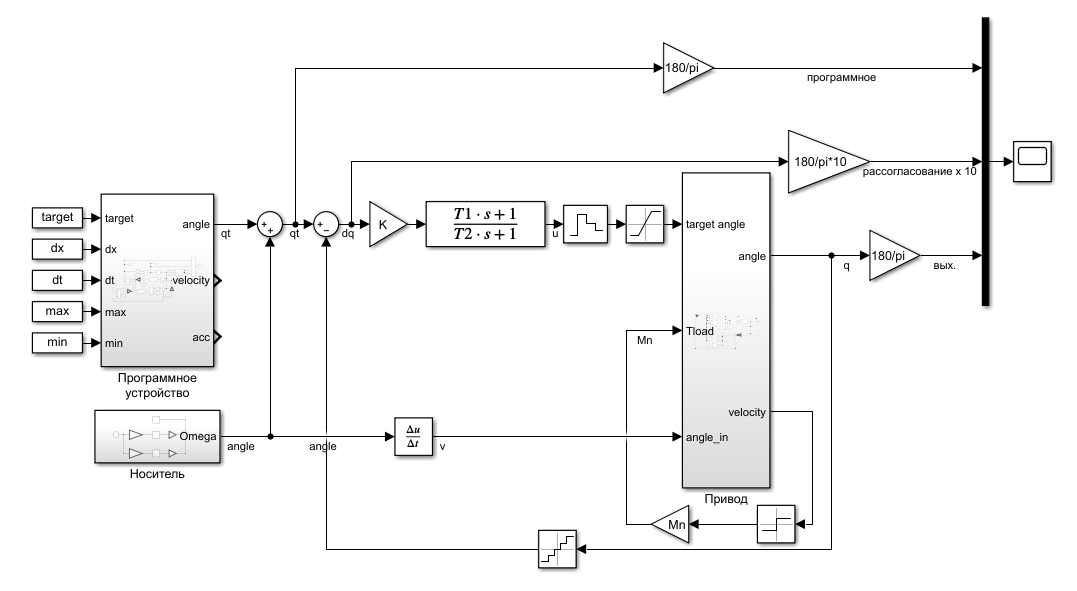
\includegraphics[width=1.0\linewidth]{system} 
 	\caption{Процессы наведения ОЭП по каналу азимута}
 	\label{fig:az_true}
\end{figure}



\begin{figure}[ht]
	\centering
	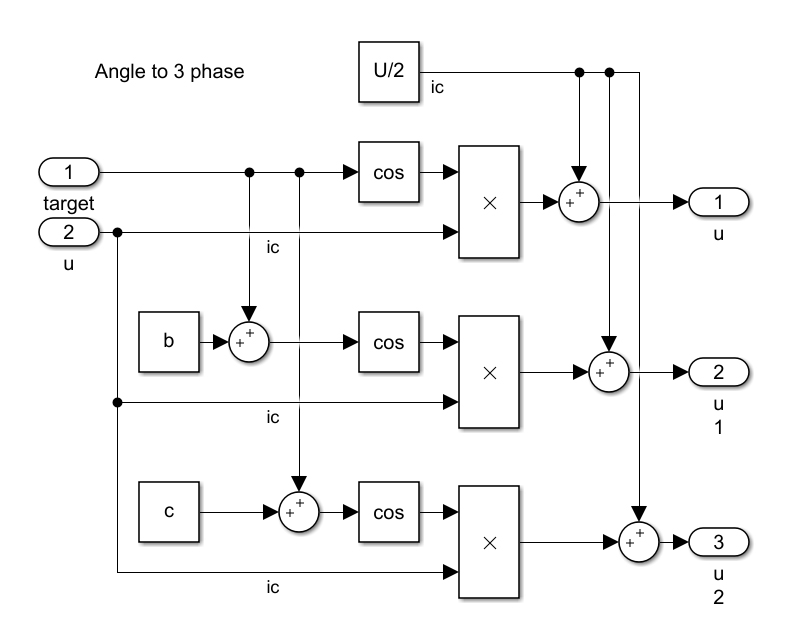
\includegraphics[width=1.0\linewidth]{A23P} 
	\caption{Процессы наведения ОЭП по каналу азимута}
	\label{fig:az_true}
\end{figure}


















\section{КИМ САУ ОЭП (схема, обозначения и…) } \label{ch:ch5/sect2}

\begin{figure}[ht]
	\centering
	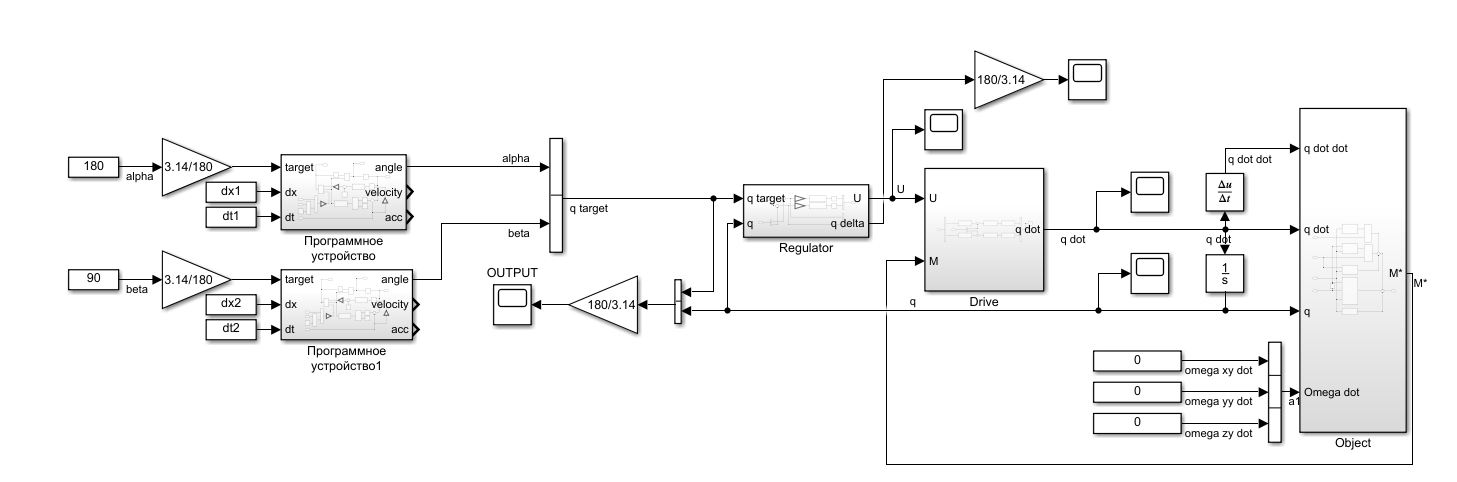
\includegraphics[width=1.0\linewidth]{C5_1} 
	\caption{Процессы наведения ОЭП по каналу азимута}
	\label{fig:az_true}
\end{figure}


\section{Разработка компьютерной имитационной модели ЦСАУ ОЭП с учетом  движения борта} \label{ch:ch5/sect3}



\begin{figure}[ht]
	\centering
	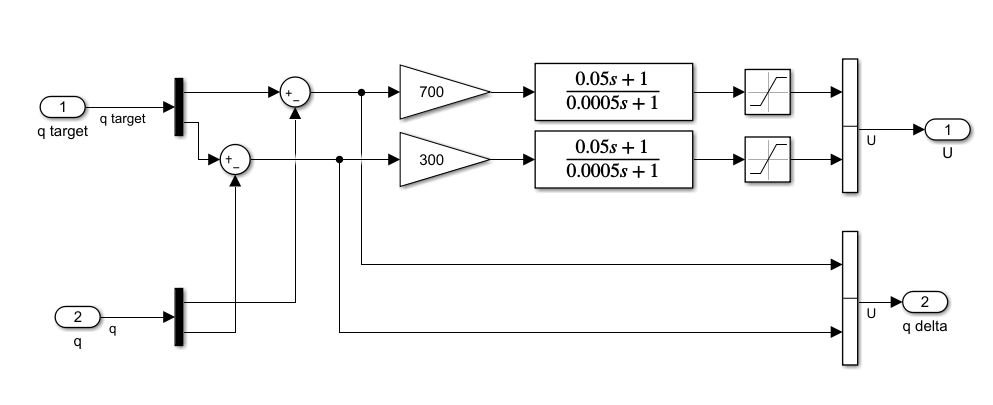
\includegraphics[width=1.0\linewidth]{C5_2} 
	\caption{Процессы наведения ОЭП по каналу азимута}
	\label{fig:az_true}
\end{figure}

\begin{figure}[ht]
	\centering
	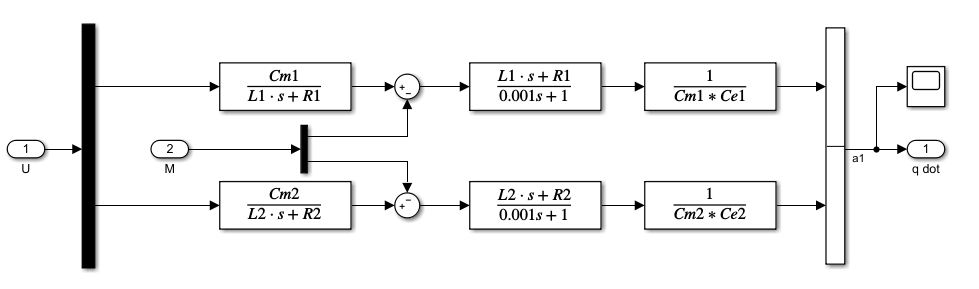
\includegraphics[width=1.0\linewidth]{C5_3} 
	\caption{Процессы наведения ОЭП по каналу азимута}
	\label{fig:az_true}
\end{figure}


\begin{figure}[ht]
	\centering
	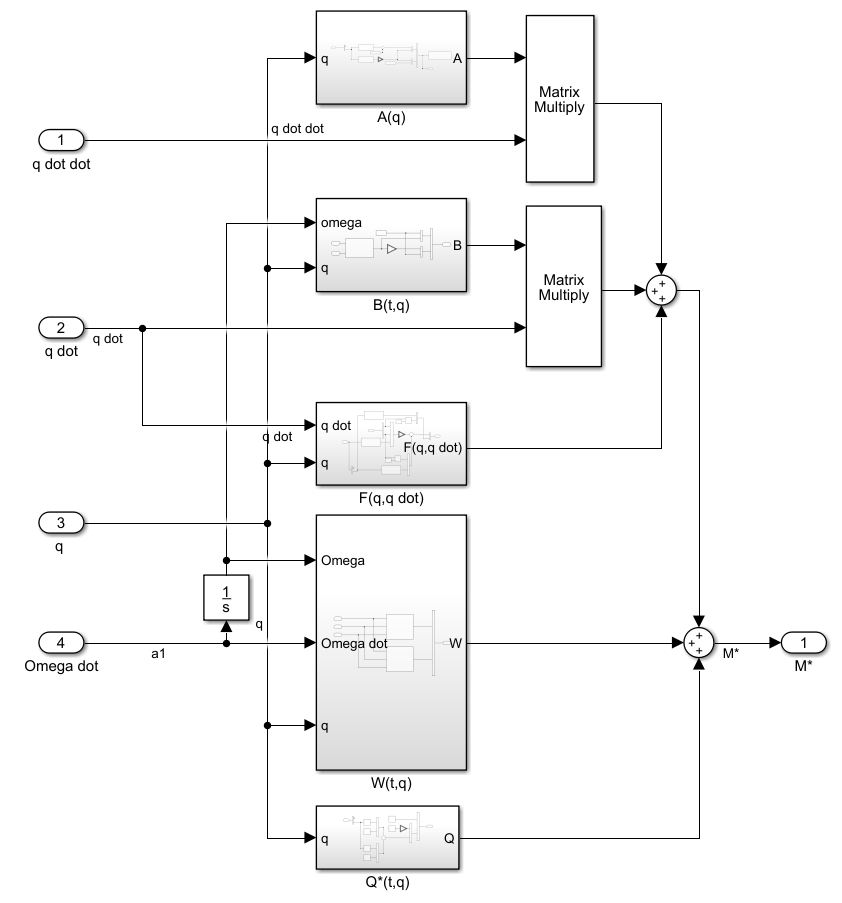
\includegraphics[width=1.0\linewidth]{C5_4} 
	\caption{Процессы наведения ОЭП по каналу азимута}
	\label{fig:az_true}
\end{figure}

\begin{figure}[ht]
	\centering
	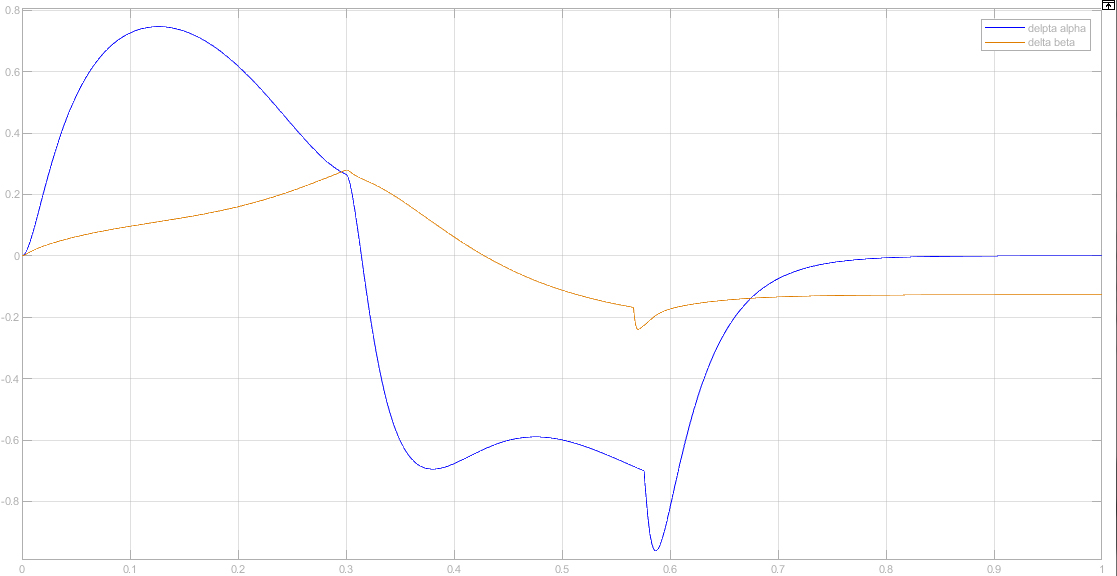
\includegraphics[width=1.0\linewidth]{C5_G1} 
	\caption{Процессы наведения ОЭП по каналу азимута}
	\label{fig:az_true}
\end{figure}
\begin{figure}[ht]
	\centering
	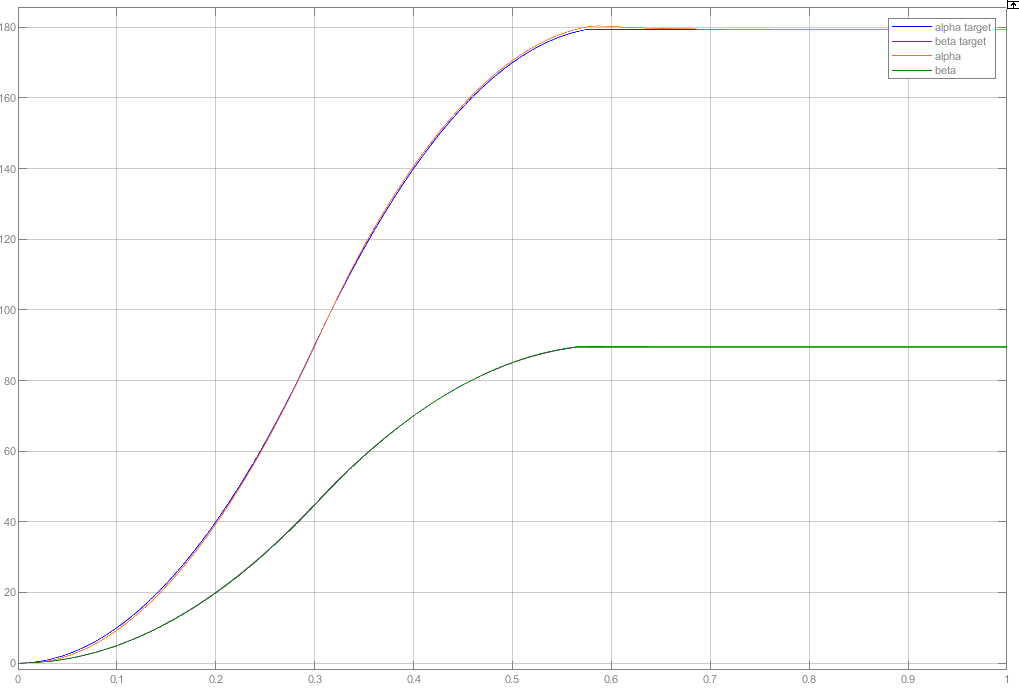
\includegraphics[width=1.0\linewidth]{C5_G2} 
	\caption{Процессы наведения ОЭП по каналу азимута}
	\label{fig:az_true}
\end{figure}

\section{Исследование динамики наведения и стабилизации ОЭП} \label{ch:ch5/sect4}

\section{Выводы} \label{ch:ch5/sect5}
	


Некоторый текст.

\clearpage